\scanpage{132}
% E24: faint, mirrored printed matter visible through the sheet.
\begin{center}\reflectbox{\begin{minipage}{.95\linewidth}\ttfamily\scriptsize\color{gray}
STMT NO. MESSAGE\par
4\quad\unsure{IEF653I} SUBSTITUTION JCL - PGM=\unsure{CRBATCH},REGION=100K,PARM=\par
\$HASP373 STARTED - INIT 10 - CLASS Q - SYS E333\par
IEF236I ALLOC. FOR CRAY2\par
IEF237I 220 ALLOCATED TO STEPLIB\par
IEF237I 4C9 ALLOCATED TO \unsure{SYS0002|SYS002}\par
IEF237I VIO ALLOCATED TO SYSUT1\par
IEF237I JES2 ALLOCATED TO SYSDUMP\par
IEF237I 79F ALLOCATED TO \unsure{CRAY}\par
IEF237I JES2 ALLOCATED TO SYSIN\par
IEF237I 79F ALLOCATED TO \unsure{SYS0012}\par
IEF237I 79F ALLOCATED TO \unsure{SYS0013|SYS0001}\par
IEF285I \unsure{CRAY2.CRAY2.JOB18231.T150735.R002}\quad CATALOGED\par
IEF285I VOL SER NOS= \unsure{CRAY11}.\par
CSS2060 - JOB QUEUED FOR TRANSFER\par
IEF142I CRAY2 CSSBATCH - STEP WAS EXECUTED - COND CODE 0000\par
IEF285I CISI.PROD.CSSBATCH.V1.\unsure{YY01}\quad KEPT\par
IEF285I VOL SER NOS= \unsure{VS004|VS104}.\par
IEF285I \unsure{SYSCINC.VSAC15}\quad KEPT\par
IEF285I VOL SER NOS= \unsure{SAC15}.\par
IEF285I \unsure{SYS82231.T150702.RA000.CRAY2.SYSUT1}\quad DELETED\par
IEF285I JES2.JOB00352.S00002\quad SYSOUT\par
IEF285I \unsure{SYS1.CR.JIF|SYSCAR.JIF}\quad KEPT\par
IEF285I VOL SER NOS= CRAY11.\par
IEF285I JES2.JOB00352.\unsure{I0101}\quad SYSIN\par
IEF285I SYS.CTLG.VCRAY11\quad KEPT\par
IEF285I VOL SER NOS= \unsure{CRAY11}.\par
IEF373I STEP /CSSBATCH/ START 82231.1507\par
IEF374I STEP /CSSBATCH/ STOP 82231.1507 CPU\quad 0MIN 00.16SEC SRB\quad 0MIN 00.02SEC VIRT\quad 84K SYS\quad\illegible{1}\par
IEF375I JOB /CRAY2\quad / START 82231.1507\par
IEF376I JOB /CRAY2\quad / STOP 82231.1507 CPU\quad 0MIN 00.16SEC SRB\quad 0MIN 00.02SEC
\end{minipage}}\end{center}

\figure{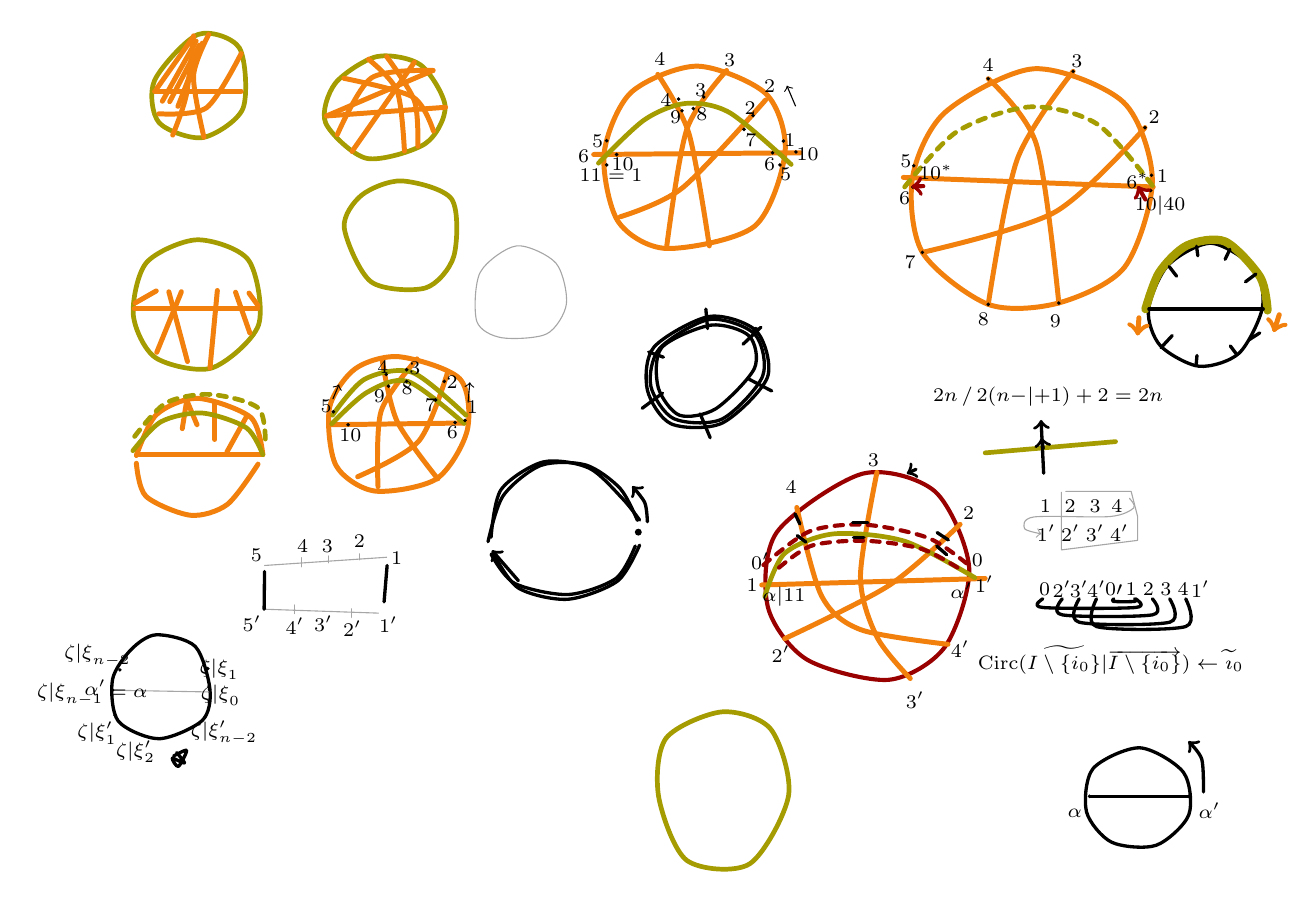
\begin{tikzpicture}[x=.55cm,y=-.55cm,line cap=round,line join=round,g/.style={olive!80!yellow,line width=1.7pt},r/.style={orange!80!brown,line width=1.8pt},w/.style={red!60!black,line width=1.5pt},b/.style={blue!60!black,line width=1.4pt},p/.style={gray!70,thin},k/.style={black,line width=1.2pt},every node/.style={font=\scriptsize}]
% E01-E06: six unlabelled small studies at left, including two empty outlines.
\draw[g] plot[smooth cycle] coordinates {(3.4,1.99) (4.36,2.3) (4.44,3.7) (3.51,4.37) (2.5,4.02) (2.4,3.05)};
\draw[r] plot[smooth] coordinates {(2.4,3.3) (4.4,3.3)};
\draw[r] plot[smooth] coordinates {(2.5,3.82) (3.6,3.68) (4.4,2.43)};
\draw[r] plot[smooth] coordinates {(3.65,1.99) (3.3,2.95) (3.54,4.36)};
\draw[r] plot[smooth] coordinates {(3.3,2.02) (3.13,3.4) (2.82,4.31)};
\draw[r] (2.45,3.24)--(3.27,2.08);
\draw[r] (2.58,3.53)--(3.36,2.14);
\draw[r] (2.75,3.54)--(3.43,2.24);
\draw[r] (2.94,3.65)--(3.5,2.19);
\draw[g] plot[smooth cycle] coordinates {(7.53,2.5) (8.54,2.69) (9.11,3.65) (8.65,4.51) (7.3,4.85) (6.35,4.03) (6.57,3.12)};
\draw[r] plot[smooth] coordinates {(6.37,3.87) (8.83,2.82)};
\draw[r] plot[smooth] coordinates {(6.37,3.87) (9.12,3.67)};
\draw[r] plot[smooth] coordinates {(6.77,3.0) (8.36,3.43) (8.84,4.22)};
\draw[r] plot[smooth] coordinates {(7.34,2.56) (8.0,3.29) (8.17,4.68)};
\draw[r] plot[smooth] coordinates {(7.76,2.5) (8.4,3.52) (8.48,4.57)};
\draw[r] plot[smooth] coordinates {(6.62,4.3) (7.41,2.99) (8.83,2.82)};
\draw[r] plot[smooth] coordinates {(6.96,4.69) (8.4,2.63)};
\draw[g] plot[smooth cycle] coordinates {(8.1,5.37) (9.26,5.79) (9.31,7.11) (8.66,7.84) (7.4,7.7) (6.78,6.45) (7.18,5.7)};
\draw[p] plot[smooth cycle] coordinates {(10.76,6.87) (11.67,7.27) (11.91,8.21) (11.46,8.9) (10.41,8.99) (9.84,8.61) (9.92,7.48)};
\draw[g] plot[smooth cycle] coordinates {(3.38,6.73) (4.57,7.2) (4.8,8.7) (3.72,9.69) (2.42,9.45) (1.91,8.47) (2.21,7.26)};
\draw[r] (1.93,8.32)--(4.78,8.32);
\draw[r] (1.95,8.19)--(2.44,7.91);
\draw[r] (2.45,9.33)--(3.02,7.93);
\draw[r] (2.73,7.93)--(3.16,9.54);
\draw[r] (3.85,7.9)--(3.68,9.69);
\draw[r] (4.27,7.94)--(4.6,8.88);
\draw[r] (4.58,7.96)--(4.79,8.25);
\draw[r] plot[smooth] coordinates {(1.98,11.71) (2.44,10.77) (3.39,10.39) (4.62,10.83) (4.9,11.69)};
\draw[r] plot[smooth] coordinates {(1.99,11.69) (4.9,11.69)};
\draw[r] plot[smooth] coordinates {(1.98,11.89) (2.2,12.65) (3.23,13.09) (4.08,12.84) (4.79,11.91)};
\draw[r] plot[smooth] coordinates {(3.14,10.46) (3.04,11.09)};
\draw[r] plot[smooth] coordinates {(3.15,10.45) (3.38,11.0)};
\draw[r] plot[smooth] coordinates {(3.79,10.49) (3.79,11.34)};
\draw[r] plot[smooth] coordinates {(4.53,10.8) (4.07,11.63)};
\draw[g] plot[smooth] coordinates {(1.9,11.6) (2.55,10.93) (3.5,10.73) (4.52,11.07) (4.9,11.69)};
\draw[g,dashed] plot[smooth] coordinates {(1.94,11.27) (2.66,10.5) (3.68,10.3) (4.8,10.62) (4.96,11.5)};
% E07: large upper-central numbered arrangement.
\draw[r] plot[smooth cycle] coordinates {(14.93,2.72) (16.52,3.36) (16.96,4.7) (16.25,6.42) (14.22,6.93) (13.1,6.3) (12.78,4.74) (13.4,3.33)};
\draw[r] plot[smooth] coordinates {(14.02,2.91) (14.74,4.28) (15.21,6.87)};
\draw[r] plot[smooth] coordinates {(15.61,2.82) (14.69,4.18) (14.22,6.93)};
\draw[r] plot[smooth] coordinates {(13.15,6.2) (14.59,5.53) (16.51,3.5)};
\draw[r] plot[smooth] coordinates {(12.54,4.76) (17.31,4.72)};
\draw[g] plot[smooth] coordinates {(12.65,4.96) (13.71,3.96) (14.67,3.58) (15.69,3.8) (17.1,4.99)};
\draw[->] plot[smooth] coordinates {(17.2,3.64) (17.0,3.17)};
\fill[black] (12.84,4.44) circle (.045);
\fill[black] (13.07,4.76) circle (.045);
\fill[black] (12.84,5.0) circle (.045);
\fill[black] (14.58,3.75) circle (.045);
\fill[black] (14.84,3.7) circle (.045);
\fill[black] (15.08,3.43) circle (.045);
\fill[black] (14.5,3.48) circle (.045);
\fill[black] (16.22,3.86) circle (.045);
\fill[black] (16.01,4.18) circle (.045);
\fill[black] (16.92,4.45) circle (.045);
\fill[black] (16.67,4.72) circle (.045);
\fill[black] (16.84,5.0) circle (.045);
\fill[black] (17.21,4.7) circle (.045);
\node at (12.63,4.46) {$5$};
\node at (12.31,4.8) {$6$};
\node at (12.94,5.24) {$11=1$};
\node at (13.21,4.98) {$10$};
\node at (14.43,3.91) {$9$};
\node at (15.04,3.84) {$8$};
\node at (16.17,4.42) {$7$};
\node at (16.6,4.98) {$6$};
\node at (16.97,5.21) {$5$};
\node at (17.07,4.42) {$1$};
\node at (17.48,4.75) {$10$};
\node at (16.15,3.7) {$2$};
\node at (16.6,3.18) {$2$};
\node at (15.01,3.27) {$3$};
\node at (15.68,2.58) {$3$};
\node at (14.21,3.5) {$4$};
\node at (14.07,2.57) {$4$};
% E08: upper-right arrangement, boundary numbering and starred labels.
\draw[r] plot[smooth cycle] coordinates {(22.71,2.78) (24.77,3.55) (25.44,5.35) (24.8,7.36) (23.27,8.19) (21.65,8.22) (20.13,7.02) (19.9,5.3) (20.65,3.79)};
\draw[r] plot[smooth] coordinates {(21.65,3.01) (22.76,4.52) (23.28,8.19)};
\draw[r] plot[smooth] coordinates {(23.61,2.84) (22.32,4.87) (21.65,8.22)};
\draw[r] plot[smooth] coordinates {(20.13,7.02) (23.19,6.09) (25.27,4.14)};
\draw[r] plot[smooth] coordinates {(19.69,5.29) (25.46,5.51)};
\draw[g,dashed] plot[smooth] coordinates {(19.72,5.51) (20.93,4.23) (22.62,3.66) (24.17,4.06) (25.46,5.5)};
\fill[black] (21.65,3.01) circle (.045);
\fill[black] (23.61,2.84) circle (.045);
\fill[black] (25.27,4.14) circle (.045);
\fill[black] (25.42,5.24) circle (.045);
\fill[black] (25.4,5.59) circle (.045);
\fill[black] (19.93,5.02) circle (.045);
\fill[black] (19.91,5.51) circle (.045);
\fill[black] (20.13,7.02) circle (.045);
\fill[black] (21.65,8.22) circle (.045);
\fill[black] (23.28,8.19) circle (.045);
\node at (21.65,2.71) {$4$};
\node at (23.7,2.61) {$3$};
\node at (25.48,3.9) {$2$};
\node at (25.67,5.26) {$1$};
\node at (25.62,5.94) {$\unsure{10|40}$};
\node at (19.75,4.91) {$5$};
\node at (19.72,5.76) {$6$};
\node at (19.85,7.24) {$7$};
\node at (21.54,8.56) {$8$};
\node at (23.2,8.62) {$9$};
\node at (20.44,5.17) {$10^*$};
\node at (25.1,5.37) {$6^*$};
\draw[w,->] plot[smooth] coordinates {(20.15,5.49) (19.88,5.5)};
\draw[w,->] plot[smooth] coordinates {(25.28,5.8) (25.1,5.49)};
% E09: small right circular count, marks and two orange arrows.
\draw[k] plot[smooth cycle] coordinates {(26.8,6.81) (27.8,7.4) (27.98,8.3) (27.44,9.35) (26.52,9.65) (25.62,9.17) (25.35,8.35) (25.8,7.32)};
\draw[g,line width=3pt] plot[smooth] coordinates {(25.28,8.33) (25.6,7.48) (26.24,6.86) (27.12,6.77) (27.93,7.59) (28.1,8.36)};
\draw[k] (25.36,8.33)--(28.0,8.33);
\draw[k] (25.83,7.35)--(26.0,7.57);
\draw[k] (26.46,6.88)--(26.49,7.1);
\draw[k] (27.23,6.95)--(27.12,7.18);
\draw[k] (27.83,7.52)--(27.59,7.7);
\draw[k] (27.92,8.88)--(27.67,9.04);
\draw[k] (27.39,9.38)--(27.24,9.18);
\draw[k] (26.45,9.63)--(26.47,9.4);
\draw[k] (25.64,9.22)--(25.9,8.94);
\draw[r,->] plot[smooth] coordinates {(25.13,8.53) (25.1,8.94)};
\draw[r,->] plot[smooth] coordinates {(28.37,8.46) (28.24,8.86)};
% E10: mid-left second numbered arrangement.
\draw[r] plot[smooth cycle] coordinates {(8.05,9.43) (9.45,9.94) (9.62,11.13) (8.91,12.25) (7.48,12.53) (6.59,11.94) (6.44,10.61) (7.03,9.71)};
\draw[r] plot[smooth] coordinates {(7.66,9.53) (8.0,10.92) (8.94,12.25)};
\draw[r] plot[smooth] coordinates {(8.46,9.48) (7.63,10.69) (7.56,12.43)};
\draw[r] plot[smooth] coordinates {(7.09,12.2) (8.5,11.38) (9.17,9.78)};
\draw[r] plot[smooth] coordinates {(6.45,11.0) (9.56,10.96)};
\draw[g] plot[smooth] coordinates {(6.51,10.78) (7.25,9.95) (8.35,9.79) (9.59,10.78)};
\draw[g] plot[smooth] coordinates {(6.49,10.98) (7.31,10.25) (8.25,10.0) (9.55,10.97)};
\draw[->] plot[smooth] coordinates {(6.52,10.4) (6.66,10.07)};
\draw[->] plot[smooth] coordinates {(9.64,10.48) (9.68,10.02)};
\fill[black] (6.53,10.7) circle (.045);
\fill[black] (6.87,11.0) circle (.045);
\fill[black] (7.75,9.84) circle (.045);
\fill[black] (7.8,10.11) circle (.045);
\fill[black] (8.22,9.73) circle (.045);
\fill[black] (8.22,10.0) circle (.045);
\fill[black] (9.09,10.0) circle (.045);
\fill[black] (8.89,10.43) circle (.045);
\fill[black] (9.34,10.95) circle (.045);
\fill[black] (9.57,10.9) circle (.045);
\node at (6.36,10.57) {$5$};
\node at (6.92,11.24) {$10$};
\node at (7.59,10.34) {$9$};
\node at (8.23,10.16) {$8$};
\node at (8.77,10.54) {$7$};
\node at (9.28,11.17) {$6$};
\node at (9.74,10.59) {$1$};
\node at (9.27,10.03) {$2$};
\node at (8.41,9.7) {$3$};
\node at (7.67,9.67) {$4$};
% E11 and E12: black circular studies with ticks, dot and directed arcs.
\draw[k] plot[smooth cycle] coordinates {(15.21,8.5) (16.3,8.84) (16.55,9.91) (15.51,10.96) (14.33,10.98) (13.78,10.2) (13.93,9.21)};
\draw[k] plot[smooth cycle] coordinates {(15.25,8.7) (16.13,8.95) (16.25,9.7) (15.36,10.63) (14.52,10.78) (14.03,10.14) (14.11,9.22)};
\draw[k] plot[smooth cycle] coordinates {(15.21,8.57) (16.26,8.91) (16.44,9.88) (15.5,10.87) (14.39,10.86) (13.86,10.11) (14.06,9.24)};
\draw[k] (13.81,9.32)--(14.15,9.44);
\draw[k] (15.13,8.33)--(15.17,8.78);
\draw[k] (15.0,10.75)--(15.23,11.3);
\draw[k] (13.66,10.62)--(14.13,10.27);
\draw[k] (16.13,9.95)--(16.65,10.22);
\draw[k] (15.99,9.14)--(16.4,8.75);
\fill[black] (16.28,8.82) circle (.08);
\draw[k] plot[smooth] coordinates {(10.1,13.7) (10.45,12.64) (11.32,11.94) (12.36,11.93) (13.15,12.47) (13.55,13.21)};
\draw[k] plot[smooth] coordinates {(13.6,13.78) (13.09,14.61) (11.94,15.03) (10.8,14.77) (10.21,13.95)};
\draw[k] plot[smooth] coordinates {(10.17,13.6) (10.4,12.5) (11.37,11.86) (12.43,12.0) (13.2,12.7) (13.6,13.2)};
\draw[k] plot[smooth] coordinates {(13.5,13.8) (13.05,14.55) (11.95,14.92) (10.71,14.66) (10.17,13.99)};
\draw[k,->] plot[smooth] coordinates {(13.78,13.24) (13.72,12.8) (13.43,12.42)};
\draw[k,->] plot[smooth] coordinates {(10.8,14.6) (10.19,13.9)};
\fill[black] (13.57,13.48) circle (.08);
% E13: middle-right divided count and crossing arrows.
\node at (23.03,10.35) {$2n\,/\,2(n\unsure{-|+}1)+2=2n$};
\draw[g] (21.58,11.65)--(24.59,11.39);
\draw[k,->] (22.93,12.12)--(22.87,10.89);
\draw[k,->] (22.92,11.55)--(22.88,11.3);
% E14: lower central coloured circle with primed numbers.
\draw[w] plot[smooth cycle] coordinates {(18.75,12.13) (20.42,12.54) (21.21,14.3) (20.65,16.13) (19.35,16.89) (17.46,16.42) (16.56,15.2) (16.77,13.48)};
\draw[r] plot[smooth] coordinates {(17.23,12.91) (17.8,14.95) (18.7,15.73) (20.72,16.07)};
\draw[r] plot[smooth] coordinates {(19.08,12.1) (18.7,14.5) (19.08,15.9) (19.85,16.86)};
\draw[r] plot[smooth] coordinates {(16.95,15.94) (19.36,14.71) (21.0,13.3)};
\draw[r] plot[smooth] coordinates {(16.42,14.7) (21.58,14.55)};
\draw[g] plot[smooth] coordinates {(16.49,14.96) (16.95,13.97) (18.08,13.52) (19.72,13.69) (21.34,14.53)};
\draw[w,dashed] plot[smooth] coordinates {(16.46,14.24) (17.53,13.46) (18.82,13.31) (20.28,13.62) (21.22,14.26)};
\draw[w,dashed] plot[smooth] coordinates {(16.82,14.3) (17.58,13.79) (18.81,13.68) (20.12,13.87) (21.07,14.38)};
\draw[k] (17.19,13.06)--(17.3,13.29);
\draw[k] (17.24,13.56)--(17.44,13.71);
\draw[k] (18.52,13.26)--(18.87,13.26);
\draw[k] (18.54,13.61)--(18.78,13.61);
\draw[k] (20.47,13.49)--(20.73,13.66);
\draw[k] (20.46,13.8)--(20.69,14.0);
\draw[k,->] plot[smooth] coordinates {(19.98,12.03) (19.77,12.13)};
\node at (17.1,12.45) {$4$};
\node at (19.0,11.82) {$3$};
\node at (21.2,13.04) {$2$};
\node at (21.4,14.12) {$0$};
\node at (21.56,14.68) {$1'$};
\node at (21.0,16.18) {$4'$};
\node at (19.96,17.36) {$3'$};
\node at (16.86,16.3) {$2'$};
\node at (16.2,14.7) {$1$};
\node at (16.39,14.15) {$0'$};
\node at (16.93,14.96) {$\unsure{\alpha|11}$};
\node at (21.03,14.83) {$\unsure{\alpha'}$};
% E15: left rectangular numbered strip.
\draw[p] (4.94,14.25)--(7.76,14.06);
\draw[p] (4.94,15.26)--(7.57,15.35);
\draw[k] (4.94,14.39)--(4.93,15.26);
\draw[k] (7.77,14.25)--(7.7,15.09);
\draw[p] (5.8,14.07)--(5.8,14.28);
\draw[p] (6.42,14.03)--(6.42,14.19);
\draw[p] (7.14,13.98)--(7.14,14.12);
\draw[p] (5.64,15.16)--(5.64,15.36);
\draw[p] (6.94,15.25)--(6.94,15.45);
\node at (4.75,14.02) {$5$};
\node at (5.82,13.81) {$4$};
\node at (6.39,13.8) {$3$};
\node at (7.13,13.69) {$2$};
\node at (7.99,14.08) {$1$};
\node at (4.65,15.59) {$5'$};
\node at (5.64,15.65) {$4'$};
\node at (6.3,15.6) {$3'$};
\node at (6.97,15.71) {$2'$};
\node at (7.8,15.62) {$1'$};
% E16: left lower circle with indexed Greek labels.
\draw[k] plot[smooth cycle] coordinates {(2.44,15.85) (3.34,16.12) (3.68,17.12) (3.5,17.83) (2.5,18.25) (1.56,17.84) (1.43,16.88) (1.86,16.19)};
\draw[p] (1.43,17.13)--(3.66,17.17);
\fill[black] (1.43,17.13) circle (.045);
\fill[black] (1.49,17.71) circle (.045);
\fill[black] (1.6,16.66) circle (.045);
\fill[black] (3.63,16.63) circle (.045);
\fill[black] (3.67,17.12) circle (.045);
\fill[black] (3.57,17.74) circle (.045);
\node at (1.08,16.32) {$\unsure{\zeta|\xi}_{n-2}$};
\node at (.96,17.23) {$\unsure{\zeta|\xi}_{n-1}=\unsure{\alpha}$};
\node at (1.03,17.07) {$\unsure{\alpha'}$};
\node at (1.07,18.12) {$\unsure{\zeta|\xi}'_1$};
\node at (1.96,18.55) {$\unsure{\zeta|\xi}'_2$};
\node at (3.89,16.64) {$\unsure{\zeta|\xi}_1$};
\node at (3.92,17.25) {$\unsure{\zeta|\xi}_0$};
\node at (4.0,18.11) {$\unsure{\zeta|\xi}'_{n-2}$};
\draw[k] plot[smooth] coordinates {(2.84,18.65) (3.14,18.52) (2.95,18.89) (2.81,18.7) (3.09,18.81) (2.91,18.57)};
% E17-E18: two order diagrams, and the arrowed circle at bottom right.
\node at (22.97,12.88) {$1$};
\node at (23.54,12.88) {$2$};
\node at (24.12,12.88) {$3$};
\node at (24.62,12.88) {$4$};
\node at (22.99,13.5) {$1'$};
\node at (23.55,13.5) {$2'$};
\node at (24.12,13.5) {$3'$};
\node at (24.68,13.5) {$4'$};
\draw[p] (23.44,12.54)--(24.95,12.54)--(25.1,13.12)--(25.1,13.67)--(23.34,13.89)--(23.34,12.56);
\draw[p,->] plot[smooth] coordinates {(24.91,12.7) (25.01,12.92) (24.46,13.12) (22.7,13.13) (22.49,13.4) (22.88,13.52)};
\node at (22.95,14.8) {$0$};
\node at (23.349999999999998,14.8) {$2'$};
\node at (23.75,14.8) {$3'$};
\node at (24.15,14.8) {$4'$};
\node at (24.55,14.8) {$\unsure{0}\prime$};
\node at (24.95,14.8) {$1$};
\node at (25.35,14.8) {$2$};
\node at (25.75,14.8) {$3$};
\node at (26.15,14.8) {$4$};
\node at (26.55,14.8) {$1'$};
\draw[k] plot[smooth] coordinates {(22.91,15.02) (22.91,15.22) (25.05,15.22) (25.05,15.02)};
\draw[k] plot[smooth] coordinates {(23.36,15.02) (23.36,15.39) (25.44,15.39) (25.44,15.02)};
\draw[k] plot[smooth] coordinates {(23.75,15.02) (23.75,15.56) (25.84,15.56) (25.84,15.02)};
\draw[k] plot[smooth] coordinates {(24.15,15.02) (24.15,15.66) (26.21,15.66) (26.21,15.02)};
\draw[k] plot[smooth] coordinates {(24.55,15.02) (24.55,15.08) (25.03,15.08) (25.03,15.02)};
\node at (24.48,16.43) {$\mathrm{Circ}(\unsure{\widetilde{I\setminus\{i_0\}}|\overrightarrow{I\setminus\{i_0\}}})\leftarrow\widetilde{\imath}_0$};
\draw[k] plot[smooth cycle] coordinates {(25.15,18.46) (26.16,19.03) (26.28,20.01) (25.53,20.71) (24.5,20.64) (23.92,19.94) (24.07,18.94)};
\draw[k] (23.99,19.58)--(26.28,19.58);
\draw[k,->] plot[smooth] coordinates {(26.62,19.48) (26.58,18.72) (26.27,18.31)};
\fill[black] (23.99,19.58) circle (.045);
\fill[black] (26.28,19.58) circle (.045);
\node at (23.65,19.98) {$\alpha$};
\node at (26.76,19.91) {$\alpha'$};
% E19: lower central empty green outline.
\draw[g] plot[smooth cycle] coordinates {(15.5,17.63) (16.63,18.03) (17.04,19.56) (16.14,21.14) (14.69,21.06) (14.04,19.59) (14.21,18.24)};
\end{tikzpicture}}

% E20: two-arrow diagram; the overwritten sign remains marked.
\diagram{\[\begin{tikzcd}[ampersand replacement=\&,column sep=large,row sep=large]
\widetilde{\Delta}_{\widetilde{\unsure{S|s}}}\arrow[r,"\varphi_0", "\sim"']\arrow[dr,"\varphi_1"'] \& \widetilde{\Delta}'_{\widetilde{\unsure{S|s}}'_0}\unsure{.}\\
\&\widetilde{\Delta}'_{\widetilde{\unsure{S|s}}_1}\deleted{\unsure{\xi}}
\end{tikzcd}\]}
% E21: labels and sequences below the left circle.
\[1\quad2\quad3\quad4\qquad1'\quad2'\quad3'\quad4'\]
\[\unsure{\zeta|\xi}_0\quad\unsure{\zeta|\xi}_1\quad\unsure{\zeta|\xi}_2\quad\unsure{\zeta|\xi}_3=\unsure{\zeta|\xi}_{n-1}.\]
\[\alpha\quad u^n\unsure{\zeta|\xi}_0,\ u^{n+1}\unsure{\zeta|\xi}_0,\ {-}\ u^{2(n-1)-1}\unsure{\zeta|\xi}_0\]
% E22: lower central sequence, with annotation written underneath.
\[\unsure{\zeta|\xi}_0\quad\unsure{\zeta|\xi}_1\quad {-}\quad\unsure{\zeta|\xi}_{n-2}\quad\underset{u^{n-1}}{\unsure{\zeta|\xi}_{n-1}}=\unsure{\zeta|\xi}'_0\]
% E23: lower-right two sequences and separate alpha.
\[\alpha,\ u^n\unsure{\zeta|\xi}_0,\ u^{n+1}\unsure{\zeta|\xi}_0,\ {-},\ u^{2n-2}\unsure{\zeta|\xi}_0\]
\[\alpha,\]
\[\unsure{\zeta|\xi}_0\quad\unsure{\zeta|\xi}_1\quad {-}\quad\unsure{\zeta|\xi}_{n-1}\quad\unsure{\bar\zeta_n|\bar\xi_n}=\unsure{\zeta|\xi}'_0\]
\margin{\mspage{131}}
